\subsection{Ejercicio 16}
\graphicspath{ {img/16} }


Antes de realizar el proceso con la VPN de la UDC, comprobamos nuestras direcciones IP privada y pública junto con la calidad de la conexión de la misma manera que en el ejercicio anterior. Mostraremos las características en las figuras \ref{fig:IPs-preUDC} y \ref{fig:Calidad-Conexión-preUDC}.

\begin{figure}[H]
    \centering
    \begin{subfigure}{.5\textwidth}
        \centering
        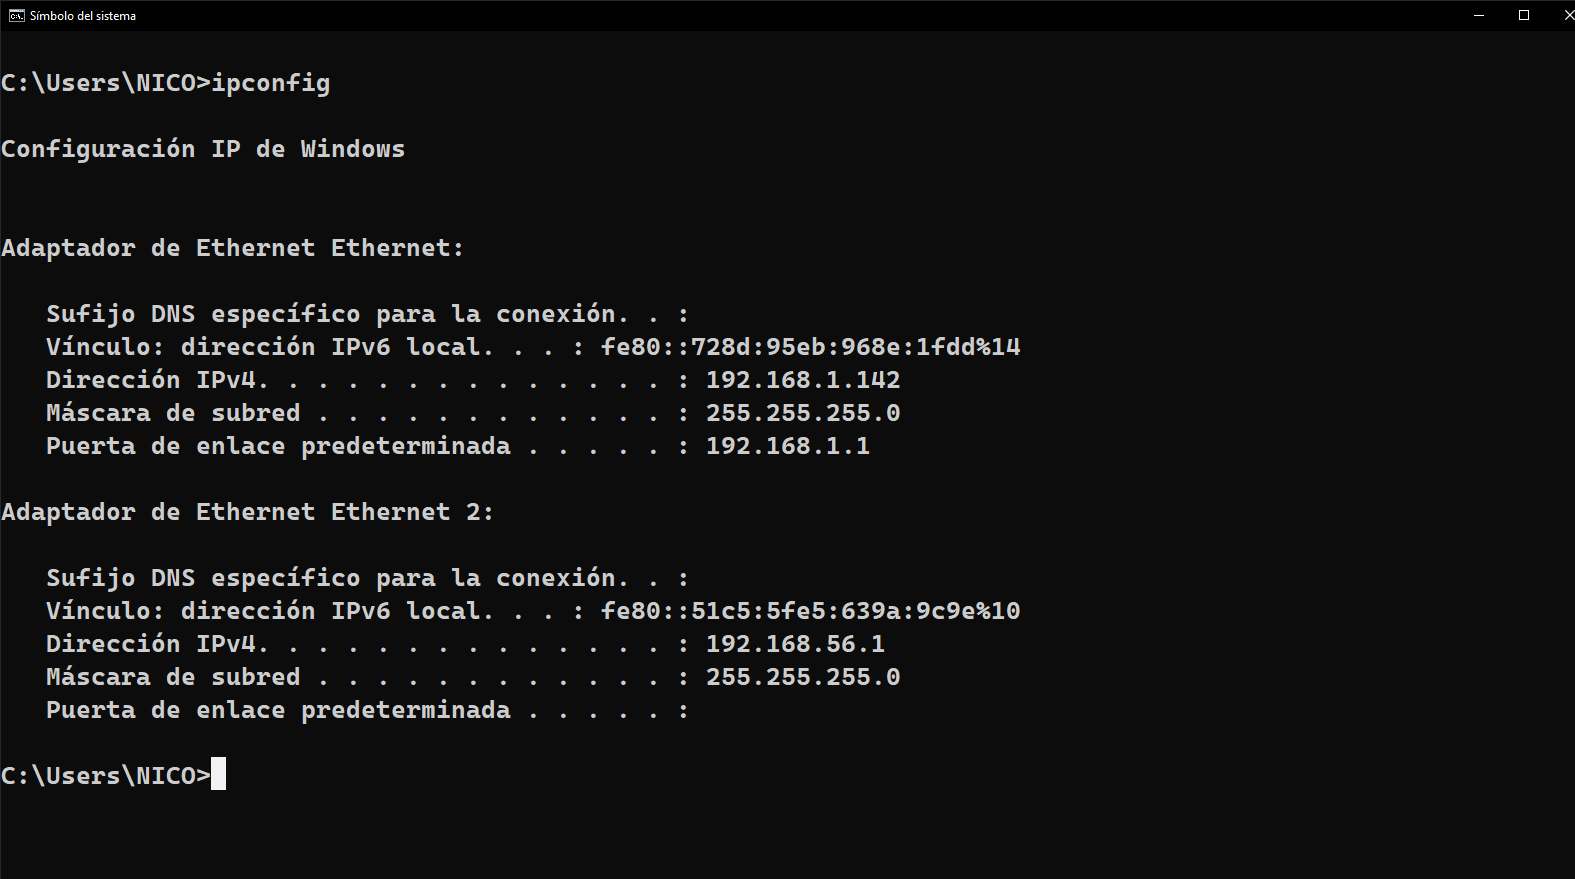
\includegraphics[width=\linewidth]{IP-Privada-preUDC.png}
        \caption{Dirección IP Privada}
    \end{subfigure}%
    \begin{subfigure}{.5\textwidth}
        \centering
        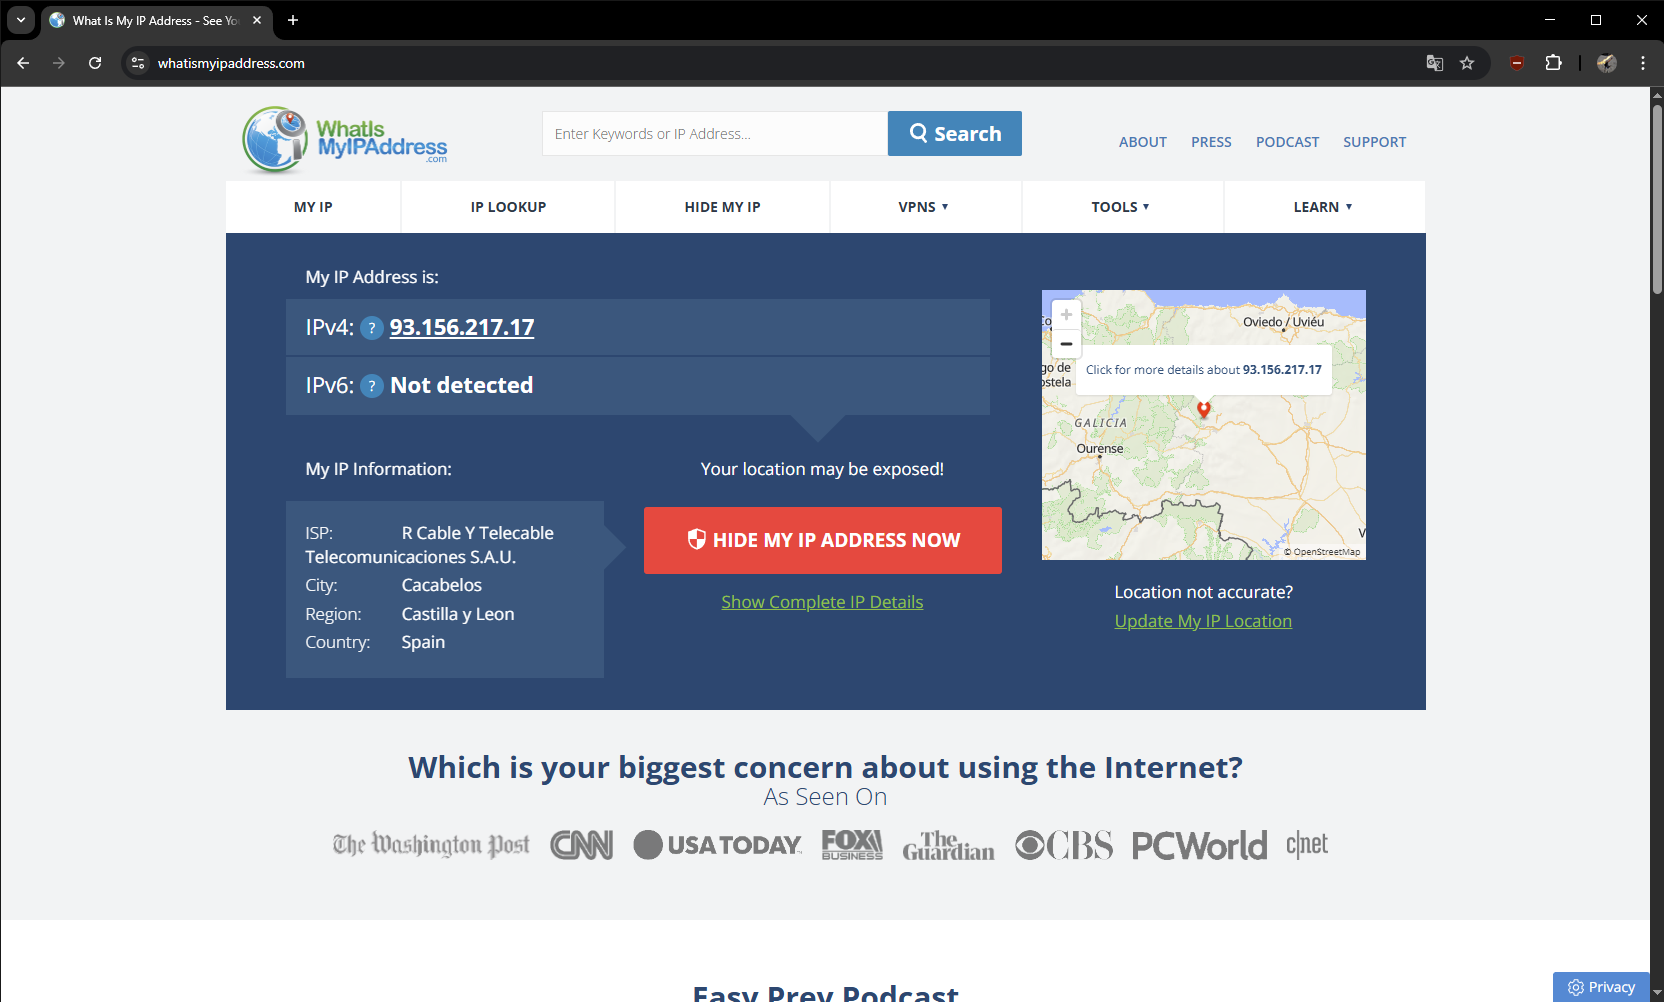
\includegraphics[width=\linewidth]{IP-Publica-preUDC.png}
        \caption{Dirección IP Pública}
    \end{subfigure}
    \caption{Direcciones IP antes de utilizar la VPN de la UDC}
    \label{fig:IPs-preUDC}
\end{figure}

\begin{figure}[H]
    \centering
    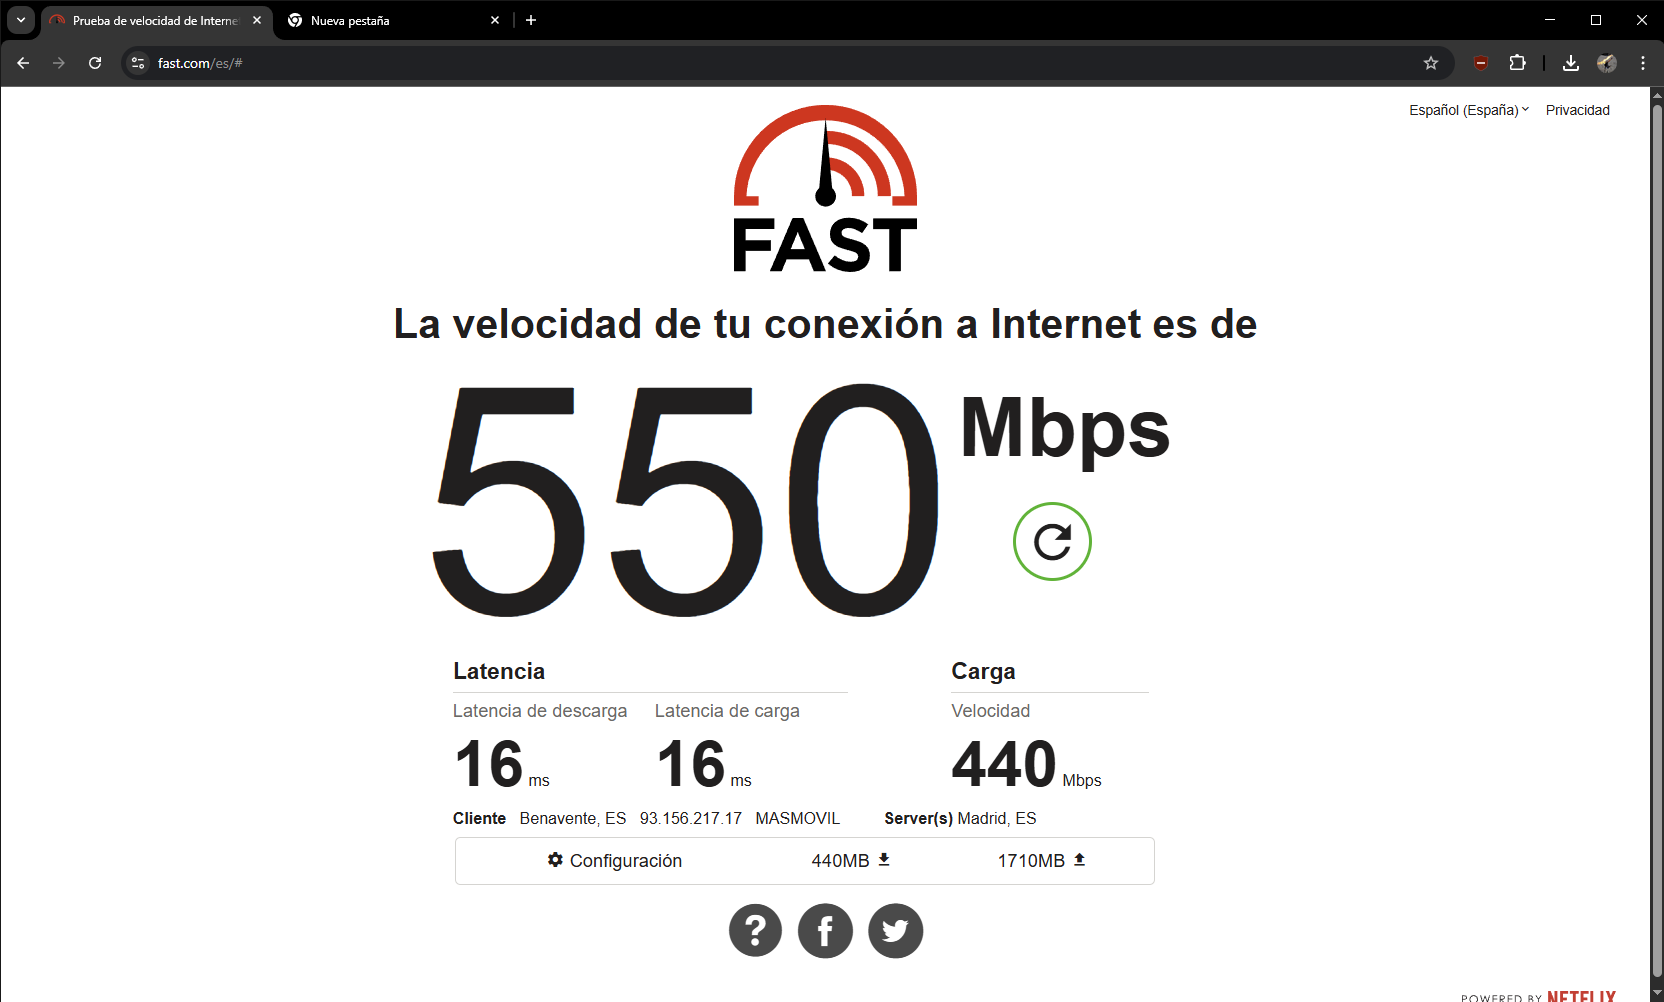
\includegraphics[width=\linewidth]{CalidadConexion-preUDC.png}
    \caption{Calidad de la conexión antes de utilizar la VPN de la UDC}
    \label{fig:Calidad-Conexión-preUDC}
\end{figure}


Observamos que las IPs privada y pública son \texttt{192.168.1.142} (primera interfaz de red) y \texttt{93.156.217.17}, respectivamente, y que contamos con una velocidad de \SI{550}{Mbps} (de descarga) y \SI{440}{Mbps} de carga, además de \SI{16}{ms} de latencia de carga/descarga.

A continuación, para poder utilizar la VPN de la UDC primero debemos instalarla y configurarla en el enlace \href{https://axudatic.udc.gal/pages/viewpage.action?pageId=45813771}{\texttt{VPN-UDC}}, dentro del apartado \texttt{`Instalación e configuración'}.

Con el cliente de VPN instalado, nos conectamos y reexaminamos los parámetros de la conexión, tal y como muestran las figuras \ref{fig:IPs-VPN-UDC} y \ref{fig:Calidad-Conexión-VPN-UDC}.

\begin{figure}[H]
    \centering
    \begin{subfigure}{.5\textwidth}
        \centering
        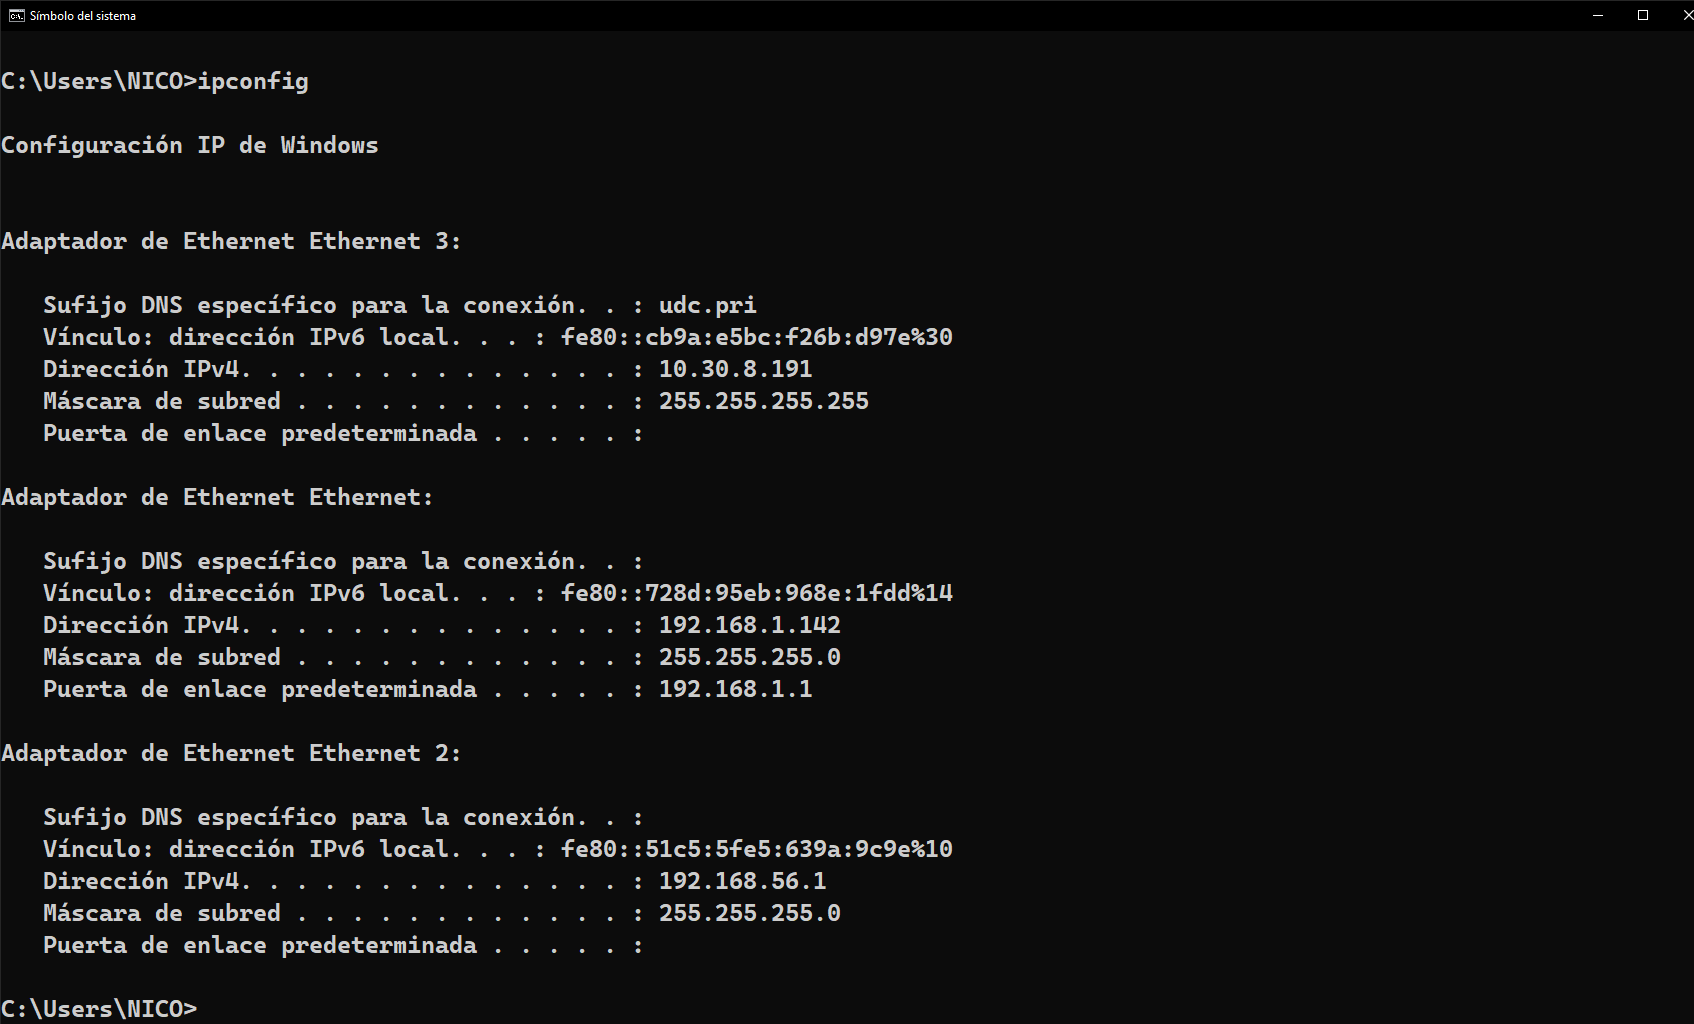
\includegraphics[width=\linewidth]{IP-Privada-VPN-UDC.png}
        \caption{Dirección IP Privada}
    \end{subfigure}%
    \begin{subfigure}{.5\textwidth}
        \centering
        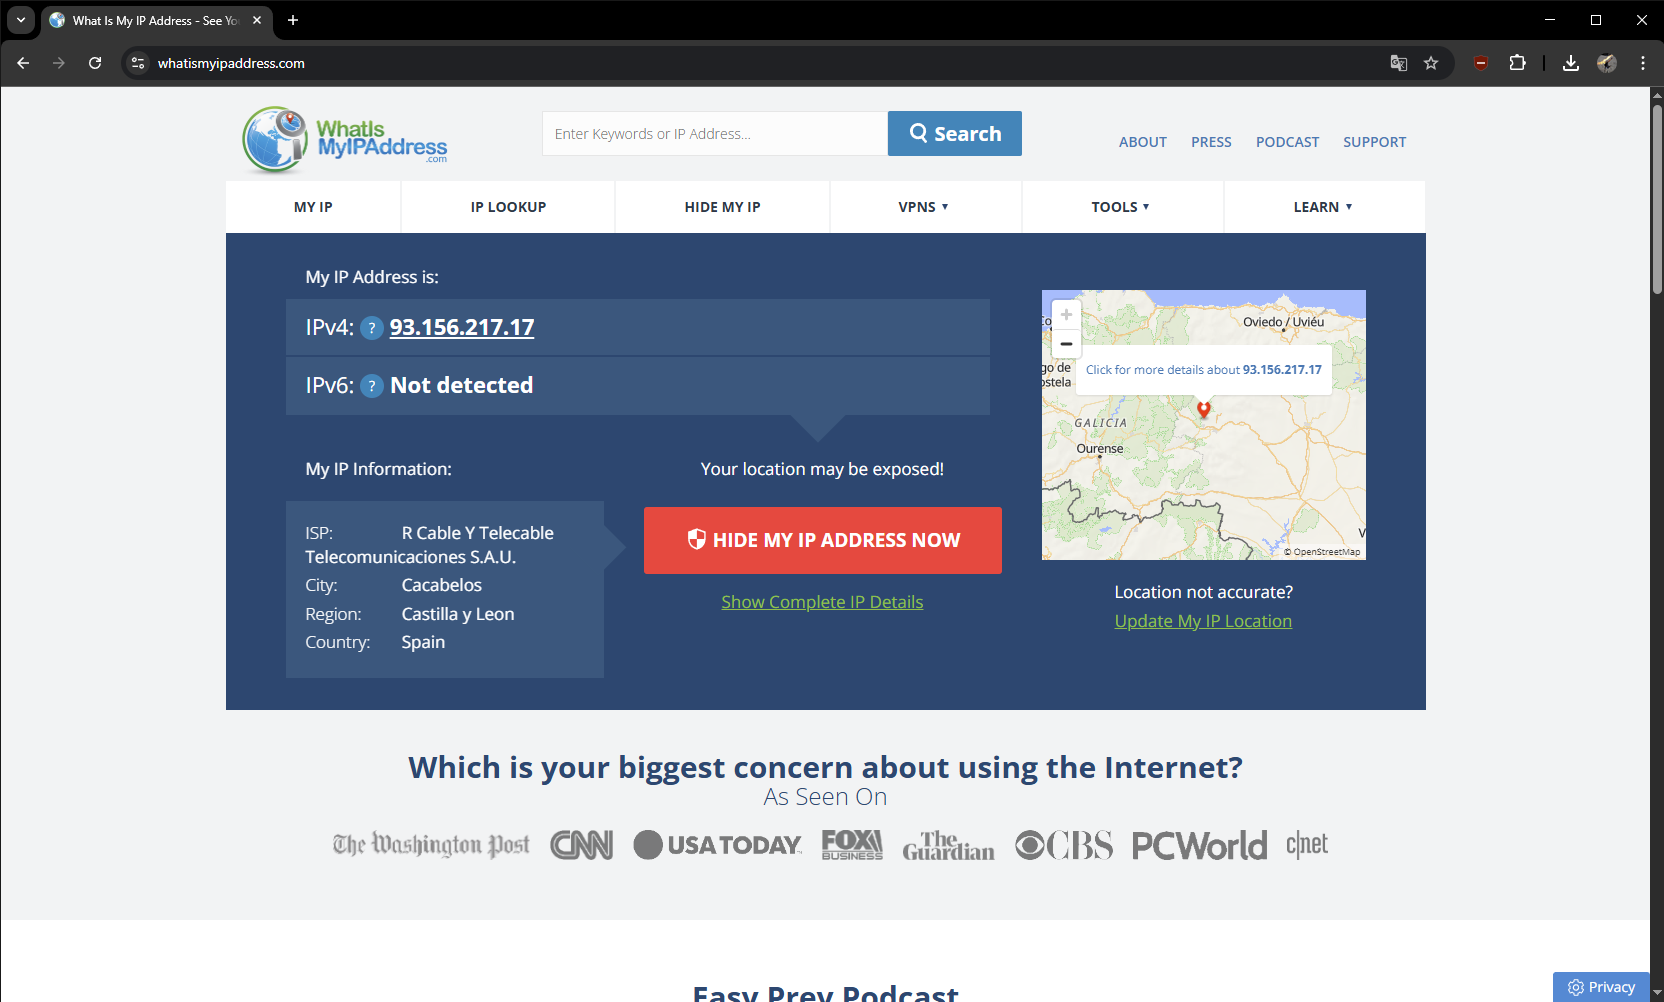
\includegraphics[width=\linewidth]{IP-Publica-VPN-UDC.png}
        \caption{Dirección IP Pública}
    \end{subfigure}
    \caption{Direcciones IP antes de utilizar la VPN de la UDC}
    \label{fig:IPs-VPN-UDC}
\end{figure}

\begin{figure}[H]
    \centering
    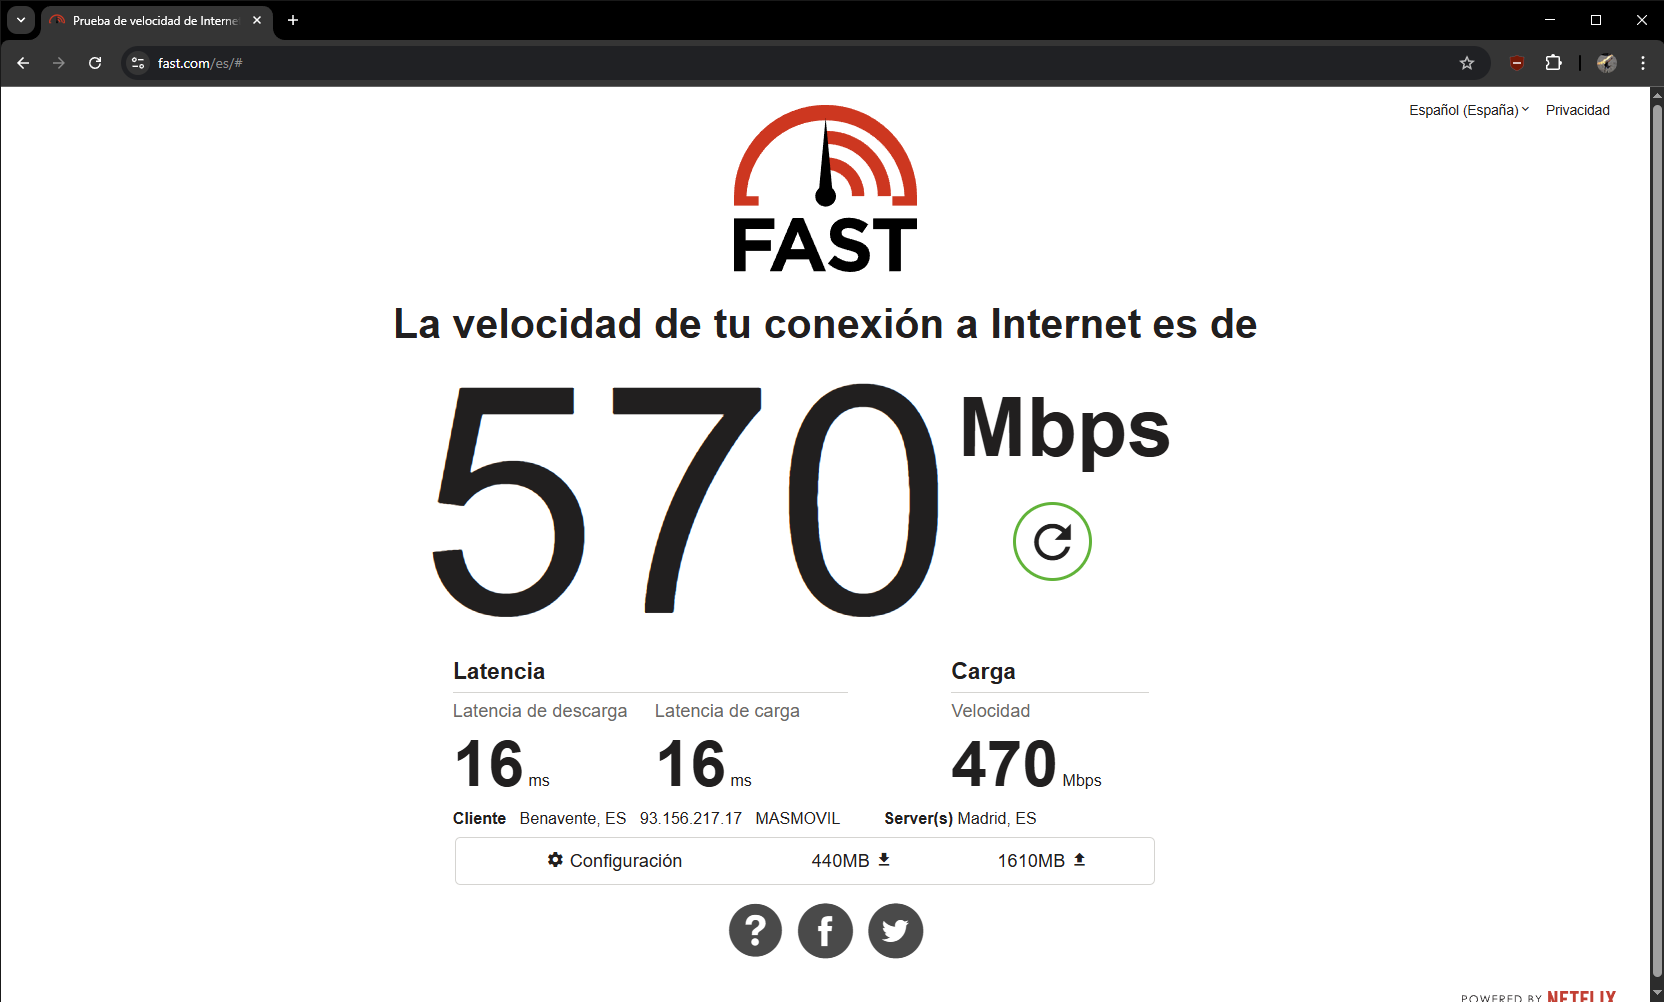
\includegraphics[width=\linewidth]{CalidadConexion-VPN-UDC.png}
    \caption{Calidad de la conexión antes de utilizar la VPN de la UDC}
    \label{fig:Calidad-Conexión-VPN-UDC}
\end{figure}

Vemos que se genera una nueva interfaz de red (que lleva el sufijo DNS \texttt{udc.pri}), que corresponde a la VPN. Su IP (privada) es \texttt{10.30.8.191/32}, sin embargo, si comprobamos la dirección IP pública utilizando un servicio web veremos la misma que antes. Esto se debe a que esta VPN no está configuarada para redirigir todo el tráfico de red por la misma.

A diferencia de ProtonVPN, la VPN de la UDC tiene como objetivo permitir el acceso desde internet a servicios que están disponibles solo desde la red de la UDC. Aunque hoy en día son extremadamente comunes las VPNs comerciales con el objetivo de enmascarar el tráfico, el de extender una red privada era el propósito original de las VPNs.

Por lo explicado anteriormente, tiene sentido el resultado observado al comprobar la velocidad de la conexión, y es que no varía, ya que para acceder al servidor web de la prueba de velocidad, que se encuentra fuera de la red de la UDC, nuestro tráfico sigue yendo de manera directa, ignorando completamente la interfaz creada por la VPN.

Si quisiéramos evaluar la calidad de esta VPN tendríamos que realizar la prueba de velocidad contra un servidor que se encuentre en la red de la UDC, ya que en este caso el tráfico sí que iría por esa interfaz y nos permitiría evaluar su calidad.
